\cxset{steward,
  chapter toc=true,
  toc image=false,
  numbering=arabic,
  custom = stewart,
  offsety=0cm,
  image={./images/hine06.jpg},
  texti={A picture is worth a thousand words, but if you don't add a good description of what it is in a caption, your readers will be left scratching their heads. Here we discuss captions in general as well as the formatting commands available in LaTeX, some common packages and athena.},
  textii={In this chapter we discuss methods that allow the formatting and positioning of captions, based on a set of key values. Central  to this process is the separation of content from presentation.
We also discuss the basic formatting tools that are available and how one can modify them to blend them with the rest of the design.
 }
}
\cxset{section numbering prefix=\thechapter.}
\chapter{Typesetting Captions}
\section{Introduction}

Publications that include figures and tables will normally dictate
the style of captions. Captions, besides normal typography 
requirements such as fonts, can vary in their numbering scheme, can
include a label such as figure or fig they can include a colon or stop
after the label and can be centered hanged or left justified. 
Numbering can also vary; the counters can be reset at every chapter or section or can be continuous. So
there are quite a few options to define in a template.

The formatting commands for the captions key value interface follow the same style of the rest of the package. We use the \pkg{caption} package to provide the interface to the key value settings. To format the captions you just include the appropriate keys in one of the style
files.


\section{Conventions}

All caption keys start with the word |caption|. The float type follows, so |caption figure font-size| refers to the caption of a \textit{figure environment}. If the word \textit{figure} is omitted the style is applicable to both tables and figures. 

As users will probably only have to set these keys once, my recommendation is to use the longer version that can give you finer control. Also your template will be easier to modify in the future.
\medskip

{
\keyval{caption format}{\marg{plain|hang}}{This affects all captions such as tables and figures and will produce either a hang caption or with plain will wrap arund the figure number like a normal paragraph.}

\keyval{caption figure format}{\marg{plain | hang}}{Affects ONLY figure captions such as tables and figures and will produce either a hang caption or with plain will wrap around the figure number like a normal paragraph.}

\keyval{caption figure numbering style}{\marg{auto|continuous|reset on sections|custom}}{}
\keyval{caption figure numbering}{\marg{arabic|alph|Alph|roman|Roman|custom}}{Sets the style of numbering.}
\keyval{caption separator}{\marg{colonsemicolon|none|custom}}{Sets the separator, such as \textbf{:} or a colon or none.}
\keyval{caption label name}{\marg{text}}{Sets the label name such as figure.}
\keyval{caption aboveskip}{\marg{dim}}{Sets the \cs{belowcaptionskip}.}
\keyval{caption belowskip}{\marg{dim}}{Sets the \cs{abovecaptionskip}. You use as simply \texttt{10pt} ot similar. In LaTeX this value is normally set as \texttt{0pt}. Note that below a float normally an additional skip is introduced.}

\keyval{caption font}{\marg{bf|tt|it}}{Sets the font commands. }
\keyval{caption figure name}{Figure}{Sets the figure name}
\keyval{caption defaults}{\marg{true|false}}{Sets all styling back to default styles.}
}

Although it looks a simple piece of text, as you notice there are about
a dozen of variables that one could set. Color can be determined both
from the caption labl colour as well as from hyperlinking if necessary.
More complicated styles can be build in a simila fashion to chapter
heads, by diverting to a custom command \cs{captionspecial}. This
will be provided at the next release of the package.


\cxset{caption format/.code=\captionsetup[figure]{format=#1}} 


\begin{texexample}{}{}
\bgroup
\cxset{caption format = hang}
\includegraphics[width=80pt]{../graphics/sudan.jpg}
\captionof{figure}{This is a very long command to see how all
these can wrap in a hang format, if the text is longer than
a paragraph.}
\egroup

\bgroup
\cxset{caption format = plain}
\captionof{figure}{This is a very long command to see how all
these can wrap in a hang format, if the text is longer than
a paragraph.}
\egroup
\end{texexample}

As you can see from the example, the changes can also be localized if
they are within a group.



\makeatletter
\def\captionlabelfont@cx{bf}
\cxset{caption font/.code = \captionsetup[figure]{font=#1}}
\cxset{caption font={bf}}
\makeatother



\begin{texexample}{}{}
\cxset{caption format = hang}
\cxset{caption font={bf}}
\captionof{figure}{This is a very long command to see how all
these can wrap in a hang format, if the text is longer than
a paragraph.}
\end{texexample}



\section{Technical discussion}

The formatting of the caption, happens in stages like the sectioning commands.  |\@makecaption|  command is responsible for the typesetting and is defined in the standard LaTeX classes. The \cs{caption} and command is defined in the LaTeX kernel in the 
|float.dtx| class. As always we will start our discussion from the user command and follow it through to the typesetting macros.

When the user command \cs{caption} is processed, LaTeX checks if it is outside a float and if it is issues an error message. It then swallows the argument. It then calls \cs{@caption} which does further processing.

\startlineat{5}
\begin{teXXX}
\def\caption{%
  \ifx\@captype\@undefined
   \@latex@error{\noexpand\caption outside float}\@ehd
   \expandafter\@gobble
 \else
   \refstepcounter\@captype
  \expandafter\@firstofone
 \fi
 {\@dblarg{\@caption\@captype}}%
}

\long\def\@caption#1[#2]#3{%
  \par
  \addcontentsline{\csname ext@#1\endcsname}{#1}%
  {\protect\numberline{\csname the#1\endcsname}{\ignorespaces  #2}}%
  \begingroup
        \@parboxrestore
  \if@minipage
     \@setminipage
  \fi
  \normalsize
 \@makecaption{\csname fnum@#1\endcsname}{\ignorespaces #3}
 \par
 \endgroup}
\end{teXXX}


The \cs{@makecaption} is the main typesetting macro and this is
where we need to hook if we want finer grain of control.

\makeatletter
\cxset{label punctuation/.code = \gdef\labelpunctuation@cx{#1}}
\cxset{label space/.code = \gdef\labelhspace@cx{\hskip#1}}
\cxset{caption above skip/.store in= \abovecaptionskip@cx}
\cxset{caption above skip=10pt}
\makeatother

\captionof{figure}{This is a very long command to see how all
these can wrap in a hang format, if the text is longer than
a paragraph.}

\begin{texexample}{}{}
\cxset{caption format = hang}
\cxset{label punctuation=?}
\cxset{label space =1.5em}
\captionof{figure}{This is a very long command to see how all
these can wrap in a hang format, if the text is longer than
a paragraph.}

\end{texexample}



\cxset{label punctuation=?}
\captionof{figure}{This is a very long command to see how all
these can wrap in a hang format, if the text is longer than
a paragraph.}

\cxset{label punctuation=:}
\cxset{label space =.5em}
\def\figurename{\textbf{Figure}}

\makeatletter
\setlength\abovecaptionskip{\abovecaptionskip@cx}
\setlength\belowcaptionskip{0\p@}

\long\def\@makecaption#1#2{%
  \vskip\abovecaptionskip
  \sbox\@tempboxa{#1\labelpunctuation@cx #2}
  \ifdim \wd\@tempboxa >\hsize
    #1\labelpunctuation@cx\labelhspace@cx#2\par
  \else
    \global \@minipagefalse
    \hb@xt@\hsize{\hfil\box\@tempboxa\hfil}%
  \fi
  \vskip\belowcaptionskip}
\makeatother

\begin{teXXX}
\newlength\abovecaptionskip
\newlength\belowcaptionskip
\setlength\abovecaptionskip{10\p@}
\setlength\belowcaptionskip{0\p@}

\long\def\@makecaption#1#2{%
  \vskip\abovecaptionskip
  \sbox\@tempboxa{#1:: #2}
  \ifdim \wd\@tempboxa >\hsize
    #1:: #2\par
  \else
    \global \@minipagefalse
    \hb@xt@\hsize{\hfil\box\@tempboxa\hfil}%
  \fi
  \vskip\belowcaptionskip}
\end{teXXX}



\section{List of Figures}

\begin{docCommand}{listoffigures}{}
The list of figures (lof) is included on a page by using the command \cs{listoffigures}.
\end{docCommand}

The command is not defined in the kernel but rather in the standard classes as shown below. By default it uses the |\chapter| to typeset its heading. Commands like |\tableofcontents| that should set the marks in some page
styles use a |\@mkboth| command, which is |\let| by the pagestyle command |(\ps@...)| to |\markboth| for setting the heading or to |\@gobbletwo| to do nothing.\footnote{See source ltpage.dtx Date: 2000/06/02 Version v1.0k, page311.}

\begin{teXXX}
\newcommand\listoffigures{%
    \if@twocolumn
      \@restonecoltrue\onecolumn
    \else
      \@restonecolfalse
    \fi
    \chapter*{\listfigurename}%
      \@mkboth{\MakeUppercase\listfigurename}%
              {\MakeUppercase\listfigurename}%
    \@starttoc{lof}%
    \if@restonecol\twocolumn\fi
    }
\end{teXXX}



In the |phd| package this is set as a property via a key-value interface and hence we can use a normal chapter. If it need be we can define a special chapter style only for this heading. This way we can control all aspects of the formatting of the head.

\begin{docCommand}{\listfigurename}{}
The \textit{List of Figures} for example in many Social Sciences books is typed as {List of Illustrations} and also adds credits.
\end{docCommand}




\begin{figure}[htp]
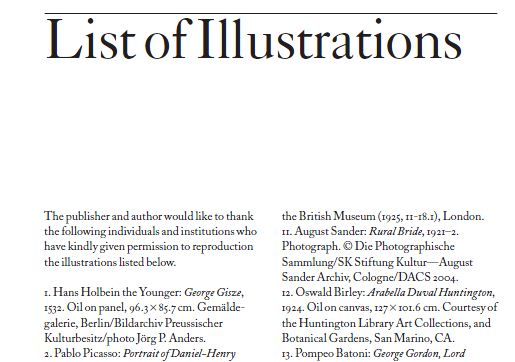
\includegraphics[width=\textwidth]{./images/listofillustrations.jpg}
\caption{List of Illustrations extract from \textit{Oxford History of Art, Portraiture}, Shearer West, Oxford University Press, 2004.}
\end{figure}
\begin{figure}[htp]
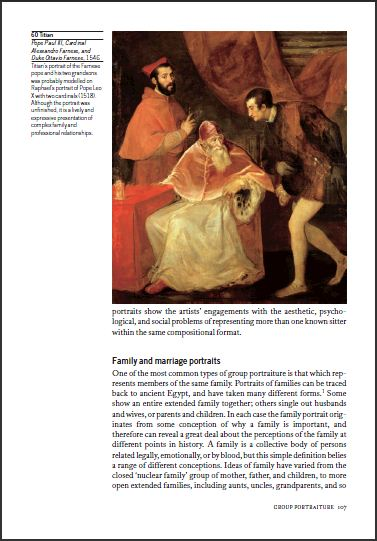
\includegraphics[width=0.67\textwidth]{./images/titian.jpg}
\centering
\caption{Figure from \textit{Oxford History of Art, Portraiture}, Shearer West, Oxford University Press, 2004. The figures are numbered consecutively and the text in the List of Illustrations have different formatting.}
\end{figure}



\section{Formatting the List of Figures Heading}

LaTeX formats the list of figures heading in a similar manner to that of the Table of Contents. The Title `List of Figures` is obtained from the \cs{listfigurename} and which is also accessible from Babel. It does not add an entry to the ToC.



It is good to know that \cs{captionsetup} has an effect on the current environment only.
So if you want to change settings for the current figure or table only, just place the
\cs{captionsetup} command inside the figure or table right before the \cs{caption}
command.


Many of the caption figures can be changed within \latexe itself. For example to get continuous numbering in the book class.

\begin{teXXX}
\makeatletter
\@removefromreset{table}{chapter}
\renewcommand{\thetable}{\arabic{table}}
\makeatother
\end{teXXX}

\begin{docCommand}{removefromreset}{}
The command \cs{removefromreset} can be found by loading the \pkg{remreset} package. Other combinations are also possible.
\end{docCommand}

\subsection{Caption numbering scheme}

The caption numbering scheme key value interface, provides five
options: 
\medskip

\keyval{caption numbering scheme}{\marg{default|continuous| chapter|section}}{The numbering style either continous or reset per spacing etc...}


\begin{comment}
% Date: Sat, 30 Jul 1994 17:58:55 PST
% From: Donald Arseneau <asnd@erich.triumf.ca>
%
%  |\@removefromreset{FOO}{BAR}| : Removes counter FOO from the list of
%                       counters |\cl@BAR| to be reset when counter BAR
%                       is stepped.  The opposite of |\@addtoreset|.
\end{comment}


\begin{teXXX}

\makeatletter
\setdefaults
\cxset{chapter opening=anywhere,
          chapter font-size=\normalfont,
          title font-size=\large}

\def\@removefromreset#1#2{\let\@tempb\@elt
   \expandafter\let\expandafter\@tempa\csname c@#1\endcsname
   
   \def\@elt##1{\expandafter\ifx\csname c@##1\endcsname\@tempa\else
         \noexpand\@elt{##1}\fi}%
   \expandafter\edef\csname cl@#2\endcsname{\csname cl@#2\endcsname}%
   \let\@elt\@tempb}

\@removefromreset{figure}{chapter}
\renewcommand{\thefigure}{\arabic{figure}}

\@specialfalse\@tocfalse
\gdef\continuousfigures@cx{\@removefromreset{figure}{chapter}
%\gdef{\thefigure}{\arabic{figure}}}

\cxset{caption numbering continuous/.code={\continuousfigures@cx}}


\chapter{This is the First Chapter}

\captionof{figure}{test}

\captionof{figure}{test}

\chapter{This is the Second Chapter}

\captionof{figure}{test}
\captionof{figure}{test}
\makeatother

\end{teXXX}


\begin{figure}[htp]
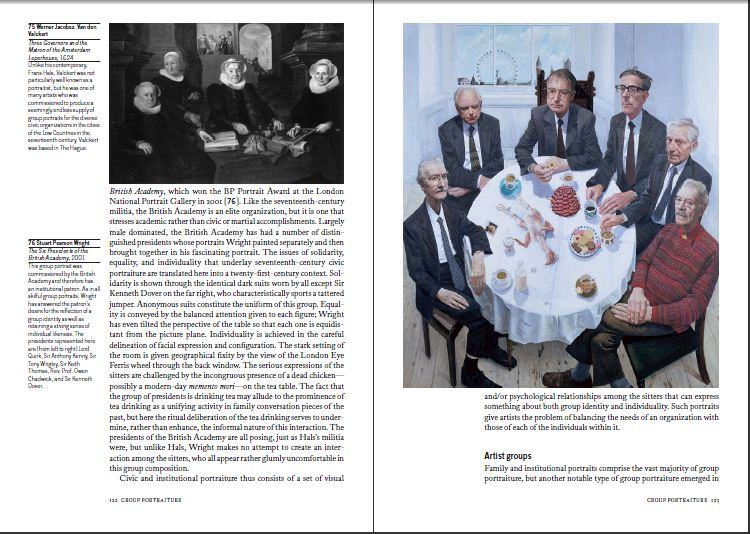
\includegraphics[width=0.98\textwidth]{./images/captionspecial.jpg}
\centering
\caption{Figure from \textit{Oxford History of Art, Portraiture}, Shearer West, Oxford University Press, 2004. The figures are numbered consecutively and the text in the List of Illustrations have different formatting.}
\end{figure}



